\documentclass[11pt,a4paper,oneside]{report}

\usepackage[utf8]{inputenc}
\usepackage[T1]{fontenc}
\usepackage[spanish,english,catalan]{babel}
\usepackage{newtxtext,newtxmath}
\usepackage{geometry}
\geometry{left=3cm,right=2.5cm,top=2.5cm,bottom=2.5cm}
\usepackage{graphicx}
\usepackage{float}
\usepackage{array}
\usepackage{longtable}
\usepackage{booktabs}
\usepackage{tabularx}
\usepackage{ragged2e}
\usepackage{caption}
\usepackage{enumitem}
\usepackage{setspace}
\usepackage{hyperref}
\usepackage{titlesec}
\usepackage{tocloft}
\usepackage{url}
\usepackage{fancyhdr}
\usepackage{etoolbox}

\hypersetup{hidelinks,pdfauthor={},pdftitle={Plantilla memoria TFG-TFM}}
\captionsetup{font={small},labelfont=bf}
\setlength{\parindent}{0pt}
\setlength{\parskip}{6pt}
\onehalfspacing
\titleformat{\chapter}[display]
  {\normalfont\huge\bfseries}
  {\chaptertitlename\ \thechapter.}{0.5em}{\Huge}
\titleformat{\section}
  {\normalfont\Large\bfseries}{\thesection}{0.75em}{}
\titleformat{\subsection}
  {\normalfont\large\bfseries}{\thesubsection}{0.75em}{}
\apptocmd{\thebibliography}{\addcontentsline{toc}{chapter}{Bibliografía}}{}{}

\renewcommand{\cftchapdotsep}{\cftdotsep}
\renewcommand{\cftchappresnum}{Capítulo\ }
\renewcommand{\cftchapaftersnum}{.\ }
\settowidth{\cftchapnumwidth}{Capítulo 10.\ }

\begin{document}
\selectlanguage{spanish}
\pagenumbering{gobble}

\begin{titlepage}
\thispagestyle{empty}
\centering
\vspace*{2cm}
{\Large\bfseries PORTADA GENERADA AUTOMÁTICAMENTE EN EBRON\par}
\vspace{1.5cm}
\begin{minipage}{0.9\textwidth}
\justifying
La aplicación EBRÓN generará automáticamente la portada de vuestra memoria en pdf y la añadirá de forma automática como primera página de la memoria. Los datos de la portada los obtendrá directamente de los datos sobre vuestro TFG/TFM que figuran en EBRÓN (título, tutores y cotutores). Así pues, es importante que eliminéis esta página de la memoria y NO incluyáis portada en el archivo pdf que depositáis. Si lo hacéis no se generará ningún error, pero vuestra memoria final incluirá dos portadas, una detrás de la otra.
\end{minipage}
\vfill

\includegraphics[width=0.78\textwidth]{images/image2.png}\par
\vspace*{1cm}
\end{titlepage}

\chapter*{Resumen}
La memoria del TFG/TFM empieza con un breve resumen de entre 250 y 830 palabras, escrito en castellano, valenciano e inglés. Estas páginas van sin numerar. Además, este deberá extender el resumen que envió como propuesta y que fue aprobado por la CAT, incluyendo los resultados y conclusiones del trabajo realizado.

\textbf{Palabras clave:}

\chapter*{Resum}
\selectlanguage{catalan}
La memòria del TFG/TFM comença amb un breu resum d’entre 250 i 830 paraules, escrit en castellà, valencià i anglès. Aquestes pàgines van sense numerar. A més, este haurà d'estendre el resum que es va enviar com a proposta i que va ser aprovat per la CAT, incloent-hi els resultats i conclusions del treball realitzat.

\textbf{Paraules clau:}

\selectlanguage{english}
\chapter*{Abstract}
The Bachelor’s Thesis/Master’s Thesis begins with a short abstract (between 250 and 830 words) written in Spanish, Valencian, and English. The cover page and the pages containing the three versions of the abstract are not numbered. In addition, the abstract must expand on the summary submitted as a proposal and approved by the CAT, including the results and conclusions of the work carried out.

\textbf{Keywords:}

\selectlanguage{spanish}
\cleardoublepage
\tableofcontents
\cleardoublepage
\listoffigures
\cleardoublepage
\listoftables
\cleardoublepage

\pagenumbering{arabic}
\setcounter{page}{6}

\chapter{Objetivo de este documento}
El objetivo de este documento es proporcionar unas directrices generales y un manual de estilo para la realización de la memoria del Trabajo Fin de Grado/Máster. Para ello, se ha detallado, a lo largo de las diferentes secciones, cuestiones importantes que se os plantean a la hora de desarrollar el trabajo. Además, se ha seguido un estilo y estructura como si de un trabajo TFG/TFM se tratara, para que así tengáis este documento como referencia/plantilla a seguir. La extensión de la memoria corresponde con la establecida en la Normativa de trabajo de fin de grado/máster del Campus de Gandia.

\chapter{Formato y estructura de la memoria}

\section{Idioma del TFG/TFM}
La memoria se podrá escribir en castellano, valenciano o inglés.

\section{Formato}

\subsection{Tipo de letra}
Se usará la fuente Times New Roman o una similar, con un tamaño mínimo de 11 puntos para el texto principal y 9 puntos para los pies de figura/tabla y las notas al pie de página.

\subsection{Párrafos}
La memoria se escribirá en párrafos justificados.

La separación entre párrafos mínima será de 6 puntos.

\subsection{Capítulos, secciones y subsecciones}
Los capítulos irán numerados y el texto se estructurará en secciones y subsecciones adecuadamente numeradas.

Los capítulos deben iniciarse siempre en una nueva página.

\section{Estructura}

\subsection{Índice}
La memoria deberá incluir un índice de todo el documento y, a continuación, se deberá incluir índices de tablas y figuras si es que la memoria incluye este tipo de elementos. Estos índices deberán generarse automáticamente a partir de los títulos y subtítulos incluidos en el propio documento.

\subsection{Figuras}
Las figuras tendrán su correspondiente numeración y texto descriptivo al pie. Deberán estar adecuadamente citadas en el texto. Además, las primeras referencias a las figuras deben estar en orden numérico (por ejemplo, en el texto no puede aparecer una referencia a la figura 2 antes de que haya aparecido la primera referencia a la figura 1). Obligatoriamente se deberá incluir la fuente de donde se ha obtenido una figura si esta no es de autoría propia. El texto descriptivo al pie de la figura debe incluir la referencia a la fuente tal y como se muestra en Figura~\ref{fig:epsg}.

\begin{figure}[H]
    \centering
    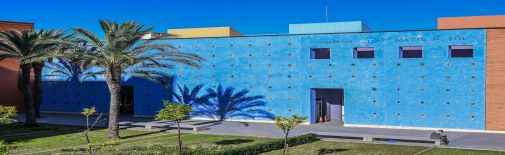
\includegraphics[width=0.82\textwidth]{images/image1.jpeg}
    \caption{Edificio A de la EPSG [Imagen]. Recuperada de \url{http://www.upv.es/contenidos/CGANDIA/}}
    \label{fig:epsg}
\end{figure}

\subsection{Tablas}
Las tablas, al igual que las figuras, tendrán su correspondiente numeración y texto descriptivo al pie y deberán estar adecuadamente citadas en el texto. Además, las primeras referencias a las tablas deben estar en orden numérico (por ejemplo, en el texto no puede aparecer una referencia a la tabla 2 antes de que haya aparecido la primera referencia a la tabla 1). Por último, las tablas seguirán una numeración independiente de la de las figuras tal y como se muestra en la Tabla~\ref{tab:ejemplo}.

\begin{table}[H]
    \centering
    \renewcommand{\arraystretch}{1.4}
    \begin{tabular}{|>{\centering\arraybackslash}m{3cm}|>{\centering\arraybackslash}m{3cm}|>{\centering\arraybackslash}m{3cm}|>{\centering\arraybackslash}m{3cm}|}
        \hline
        \textbf{Columna 1} & \textbf{Columna 2} & \textbf{Columna 3} & \textbf{Columna 4} \\
        \hline
        & & & \\
        \hline
        & & & \\
        \hline
        & & & \\
        \hline
        & & & \\
        \hline
        & & & \\
        \hline
        & & & \\
        \hline
        & & & \\
        \hline
        & & & \\
        \hline
    \end{tabular}
    \caption{Ejemplo de tabla.}
    \label{tab:ejemplo}
\end{table}

\subsection{Bibliografía}
La memoria debe incluir una relación bibliográfica de las fuentes consultadas. Las referencias bibliográficas siempre deberán estar convenientemente citadas en el texto de la memoria. El formato que se debe aplicar será el APA y deberá ser coherente en todo el documento. Se deberá dedicar una sección de esta para listarlas con la notación descrita en (Apa Style, 2023).

\subsection{Anexos}
Los anexos en formato texto y/o imagen que se hayan desarrollado en el TFG/TFM deben añadirse al final de esta memoria después de la sección de referencias bibliográficas. Además, deben estar ordenados numéricamente (Anexo 1, Anexo 2, etc.), con letras (Anexo A, Anexo B, etc.) o números romanos (Anexo I, Anexo II, etc.) y deben ir acompañados de un título (por ej. ANEXO I. Transcripción de la entrevista a Pau Donés). En esta plantilla se incluye ya el anexo que se debe incluir de forma obligatoria sobre la relación que tiene el TFG/TFM con los ODS de la agenda 2030.

Todo el material adicional que se considere necesario (por ejemplo, aplicaciones desarrolladas, listados de código, ficheros multimedia u otros archivos similares) deberá subirse a EBRÓN a través del campo “Material adicional a la memoria”. En caso de incluir varios archivos, éstos deberán agruparse y subirse en un único fichero comprimido en formato ZIP.

\section{Extensión y Apartados de la memoria}
La memoria no deberá exceder el número de páginas indicadas en la normativa para cada uno de los títulos (sin contar los anexos). Además, las páginas deberán de estar numeradas, comenzando en la página en la que se inicia el capítulo 1.

En cuanto a los apartados de la memoria, aunque estos dependerán del tipo de trabajo a desarrollar, estos deberán incluir al menos los siguientes apartados:

\textbf{Portada (aparecerá de forma automática al subirlo a EBRÓN)}

Esta no se debe elaborar ya que la genera EBRÓN automáticamente al subir la memoria. En ella se incluye los datos formales del trabajo: título, autor/a, tutores/as, titulación, universidad y año.

\textbf{Resumen}

En esta sección se deberá incluir una síntesis clara y breve del trabajo que además deberá extender el resumen que envió como propuesta y que fue aprobado por la CAT, incluyendo los resultados y conclusiones del trabajo realizado.

\textbf{Palabras clave}

Se deberá incluir entre 3 y 5 palabras que permitan identificar de inmediato de qué trata el trabajo.

\textbf{Índices}

El documento deberá incluir uno o varios índices que faciliten la navegación por el documento. Entre ellos se incluirá el índice general (capítulos y secciones), índice de figuras, índice de tablas y, si corresponde, otros índices (glosario, acrónimos, etc.).

\textbf{Introducción}

Esta sección deberá situar al lector sin necesidad de conocimientos previos profundos. Por ello, en ella se deberá presentar el contexto del trabajo y su motivación, explicando:

\begin{itemize}[leftmargin=1.3cm]
    \item Por qué es importante el tema
    \item Qué problema se quiere resolver
    \item Qué se conocerá o logrará al finalizar el documento
    \item Cómo está estructurado el TFG/TFM
\end{itemize}

\textbf{Metodología}

Esta sección deberá ser lo suficientemente detallada para que el lector pueda reproducir o entender el proceso seguido. Para ello, se deberá describir cómo se ha desarrollado el trabajo, especificando, por ejemplo:

\begin{itemize}[leftmargin=1.3cm]
    \item Técnicas, métodos o herramientas empleadas
    \item Procedimientos experimentales, analíticos o de diseño
    \item Tecnología, software, fuentes de datos, criterios de evaluación…
\end{itemize}

\textbf{Desarrollo y resultados del trabajo}

Esta sección corresponde con el cuerpo principal del TFG/TFM y la parte más extensa de este. Debe reflejar el aporte del estudiante y para ello se deberá incluir:

\begin{itemize}[leftmargin=1.3cm]
    \item Explicación detallada del trabajo realizado
    \item Análisis, experimentos, diseños, implementaciones o estudios efectuados
    \item Resultados obtenidos, presentados con claridad (tablas, gráficos, ejemplos, capturas, etc.)
    \item Interpretación o discusión de los resultados
\end{itemize}

\textbf{Conclusiones y propuesta de trabajo futuro}

En esta sección se deberá responder a los objetivos planteados, recogiendo los aprendizajes clave y el valor del trabajo realizado.

Además, se deberá incluir, si procede, el trabajo futuro propuesto, incluyendo mejoras, ampliaciones o líneas de investigación abiertas que podrían continuar el proyecto.

\textbf{Bibliografía}

En esta sección se deberá incluir un listado organizado de todas las fuentes citadas en el trabajo, como libros, artículos, webs, normativa, manuales, etc. Para ello se deberá seguir las pautas indicadas en la sección 2.3.4.

\textbf{Anexos}

En esta sección se deberá incluir un listado de todos los anexos de texto y/o imagen siguiendo las pautas indicadas en la sección 2.3.5.

\begin{thebibliography}{9}

\bibitem{apa2023}
Apa Style. (2023). \textit{Reference examples}. Recuperado en septiembre de 2023 de \url{https://apastyle.apa.org/style-grammar-guidelines/references/examples}

\bibitem{jackson2019}
Jackson, L. M. (2019). \textit{The psychology of prejudice: From attitudes to social action}. American Psychological Association.

\end{thebibliography}

\chapter*{ANEXO I. Relación del TFG/TFM con los ODS de la agenda 2030}
\addcontentsline{toc}{chapter}{ANEXO I. Relación del TFG/TFM con los ODS de la agenda 2030}

Grado de relación del trabajo con los Objetivos de Desarrollo Sostenible (ODS).

\renewcommand{\arraystretch}{1.35}
\begin{longtable}{|p{6.7cm}|>{\centering\arraybackslash}p{1.5cm}|>{\centering\arraybackslash}p{1.5cm}|>{\centering\arraybackslash}p{1.5cm}|>{\centering\arraybackslash}p{1.8cm}|}
\hline
\textbf{Objetivos de Desarrollo Sostenibles} & \textbf{Alto} & \textbf{Medio} & \textbf{Bajo} & \textbf{No procede} \\
\hline
\endfirsthead
\hline
\textbf{Objetivos de Desarrollo Sostenibles} & \textbf{Alto} & \textbf{Medio} & \textbf{Bajo} & \textbf{No procede} \\
\hline
\endhead
ODS 1.\ Fin de la pobreza. & & & & \\
\hline
ODS 2.\ Hambre cero. & & & & \\
\hline
ODS 3.\ Salud y bienestar. & & & & \\
\hline
ODS 4.\ Educación de calidad. & & & & \\
\hline
ODS 5.\ Igualdad de género. & & & & \\
\hline
ODS 6.\ Agua limpia y saneamiento. & & & & \\
\hline
ODS 7.\ Energía asequible y no contaminante. & & & & \\
\hline
ODS 8.\ Trabajo decente y crecimiento económico. & & & & \\
\hline
ODS 9.\ Industria, innovación e infraestructuras. & & & & \\
\hline
ODS 10.\ Reducción de las desigualdades. & & & & \\
\hline
ODS 11.\ Ciudades y comunidades sostenibles. & & & & \\
\hline
ODS 12.\ Producción y consumo responsables. & & & & \\
\hline
ODS 13.\ Acción por el clima. & & & & \\
\hline
ODS 14.\ Vida submarina. & & & & \\
\hline
ODS 15.\ Vida de ecosistemas terrestres. & & & & \\
\hline
ODS 16.\ Paz, justicia e instituciones sólidas. & & & & \\
\hline
ODS 17.\ Alianzas para lograr objetivos. & & & & \\
\hline
\end{longtable}

Después de rellenar la tabla deberás justificar la alineación del TFG/TFM con los ODS con un grado de relación más alto. Para ello podrás utilizar tantas páginas como sea necesario. Recuerda eliminar también este párrafo en la versión final de tu memoria.

\end{document}
